\documentclass[reprint,amsmath,amssymb,aps,prd,nofootinbib,floatfix]{revtex4-2}

\usepackage{graphicx}
\usepackage{bm}
\usepackage{physics}
\usepackage{placeins}
\usepackage[nopatch=footnote]{microtype}

% Reduce minor underfull/overfull boxes without manual line-breaking
\setlength{\emergencystretch}{2em}

\begin{document}

\title{Self-Interacting Stochastic Dynamics with Exponential Memory: Markov Embedding, Effective Scaling, and a Linear Memory-Cloud Baseline}

\author{H. Horn}
\affiliation{Peine Stederdorf, Germany}

\date{26 July 2026}

\begin{abstract}
We study a point-valued stochastic process on a continuous state space in which
a visible trajectory is coupled to a self-generated memory density with
exponential forgetting.
The visible trajectory is generally non-Markovian, whereas the augmented state
consisting of position and memory field is Markov.
The memory recursion compresses ordered histories and supplies an internal
persistence scale; a formal continuum description is available under an
explicit small-step scaling.
For the normalized memory update we derive an exact recursion for the memory
centroid and, after local linearization of the self-induced force, an
autoregressive relative mode with an explicit stationary radius.
Across nine active long-run slices, spanning $d=3$ to $20$ and run lengths up
to $3\times10^8$ updates, measured co-moving radii agree with the finite-memory
linear prediction to a median relative error of $0.76\%$ and a maximum of
$1.15\%$.
Matched one- and two-scale kernels also collapse when parametrized by local
restoring curvature.
Thus the current scalar evidence establishes a reproducible co-moving
relaxation cloud, but does not isolate a nonlinear metastable state, a phase
transition, or a dimension-selection mechanism.
\end{abstract}

\maketitle

%-------------------------------------------------
\section{Introduction}
%-------------------------------------------------

Self-interacting stochastic processes describe motion whose future drift is
shaped by its own past.
Reinforced processes, true self-avoiding or self-repelling motion, Brownian
polymers, and self-interacting diffusions provide established examples
\cite{Pemantle2007,AmitParisiPeliti1983,TothWerner1998,
DurrettRogers1992,PelitiPietronero1987}.
In the framework of Bena\"im, Ledoux, and Raimond, the interaction is driven by
a normalized occupation measure; for symmetric interactions, Bena\"im and
Raimond proved convergence toward critical points of a nonlinear free-energy
functional \cite{BenAImRaimond2002,BenaimRaimond2005}.
Herrmann and Roynette studied a different self-attracting diffusion driven by
an unnormalized integral over the full past and proved convergence or
boundedness in specific one-dimensional cases
\cite{HerrmannRoynette2003}.
These models retain cumulative rather than exponentially discounted history.

The closest recent comparison is the aging-kernel model of Mili\v{s}i\'c,
Meunier, and Roux, which treats weighted linear interactions with the past and
includes an explicitly solvable exponential-memory case
\cite{MilisicMeunierRoux2026}.
More broadly, exponential kernels admit Markovian embeddings in generalized
Langevin and other memory equations by introducing auxiliary state variables
\cite{Mori1965,Zwanzig2001,JaganathanValani2025,
WisniewskiLuczkaSpiechowicz2024}.

This paper does not claim that exponential memory or state augmentation is a
new general principle.
Its contribution is the specific combination of a discrete point process, a
deposited spatial memory field, and a potentially nonlinear self-interaction,
together with a discriminating linear center-relative null model for the
observed localized regime.
That null model materially changes the numerical interpretation: compact
co-moving scalar memory clouds are reproducible, but their measured radius is
almost completely explained by a real linear finite-memory mode.

The remainder of the paper defines the augmented process and its operator
representation, separates update order from physical time, derives the linear
null model, tests it against the current long-run data and matched controls,
and states the additional diagnostics required before using metastability or
``dynamical knot'' language.
The construction assumes neither physical spacetime nor calibrated energy,
mass, relativistic, quantum, or particle-physics structure.
\section{Minimal Dynamical Model}\label{sec:MinDynModel}
%-------------------------------------------------

In this section we define the minimal dynamical framework underlying the present paper.
No assumptions about spacetime, physical geometry, quantum mechanics, physical fields, or conserved quantities are made at this stage.

\subsection{Background structure and regularity}\label{sec:background_invariances}

For the discrete model we take $\Omega\subseteq\mathbb{R}^d$ with Lebesgue
measure and a specified boundary or extension convention.
The deposition kernel satisfies $G_\sigma\in L^1(\Omega)$,
$G_\sigma\geq0$, $\int G_\sigma=1$, and has zero first moment.
The interaction kernel $K(x,y)$ is measurable and continuously
differentiable in $x$, with $\nabla_xK(x,\cdot)$ integrable against the finite
memory measures reached by the process.
These assumptions suffice for the discrete expressions below; the formal
continuum approximation additionally requires local Lipschitz and growth
bounds on the induced drift, and the Hessian discussion requires two
$x$-derivatives near the linearization point.

The Euclidean coordinates and inner product define gradients, isotropic noise,
and covariance diagnostics.
They are part of the mathematical model and are not identified with physical
space.
Translation, rotation, and scale comparisons below refer to this supplied
coordinate scaffold.
Quantities involving $\nabla$ or a Hessian are therefore coordinate-dependent
unless combined into an explicitly normalized diagnostic.
\subsection{State and update index}

We consider a single generative process producing a sequence of states indexed by an integer update parameter $n\in\mathbb{N}$.
The parameter $n$ labels successive update steps of the process and does not represent physical time.

The full process state at update step $n$ is
\begin{equation} \label{eq:augmented_state}
z_n := (x_n,\rho_n).
\end{equation}

Here $x_n\in\Omega$ denotes the current position of the process, while $\rho_n$ is a memory density on $\Omega$ encoding the influence of past states.
The normalization condition specified below fixes the scale of the memory density and should not be read as an epistemic probability unless explicitly stated.
Given $z_n$ and a fresh noise draw $\xi_n$, the distribution of $z_{n+1}$ is determined by Eqs.~(\ref{eq:trajectory}) and~(\ref{eq:memorydistribution}).
This Markov embedding, summarized in Fig.~\ref{fig:markov_embedding}, is the Markovian description used throughout this paper.
The projected process $\{x_n\}$ alone is generally non-Markovian, because two identical visible positions with different memory densities can generate different next-step distributions.

Assumptions on $\Omega$ (continuity, reference measure, and coordinate/inner-product scaffold) were fixed in Sec.~\ref{sec:background_invariances} and are used here as an effective parametrization for writing Eqs.~(\ref{eq:trajectory})--(\ref{eq:memorypotential}). Throughout this paper, $\Omega$ remains an abstract state space; any identification with physical space or spacetime geometry is deferred to later work.

The analysis below focuses on a single generative process.
This is sufficient for the Markov embedding, the memory-induced arrow of update order, and the metastability diagnostics developed here.
Coupled multiple generators, for example through a shared memory field, are a natural extension but are not required for the construction in this paper.

\subsection{Markov kernel and observable dynamics}

Let $\Sigma$ denote the augmented state space of pairs $z=(x,\rho)$.
To make the Markov embedding explicit, and to fix the operator language used later for relaxation and metastability, we represent the one-step stochastic update by a transition kernel rather than by a deterministic map:
\begin{equation}
P(z,A)
:=
\mathbb{P}\{z_{n+1}\in A\mid z_n=z\},
\qquad
A\subseteq\Sigma .
\end{equation}
Equivalently, the dynamics acts on bounded observables $f:\Sigma\to\mathbb{R}$ through the Markov/Koopman operator
\begin{equation}\label{eq:observable_operator}
(Uf)(z)
:=
\int_\Sigma f(z')\,P(z,dz')
=
\mathbb{E}[f(z_{n+1})\mid z_n=z].
\end{equation}
This operator is linear, positive, and unital ($U1=1$), while the dual operator propagates probability measures on $\Sigma$.
The iterates satisfy the semigroup relation $U^{m+n}=U^mU^n$.
In the stochastic case $U$ is generally not multiplicative, i.e. $U(fg)$ need not equal $(Uf)(Ug)$; hence the appropriate present language is a positive Markov operator on an observable algebra, not a deterministic automorphism of that algebra.
For compact or otherwise suitably topologized state spaces, closely related algebraic formulations identify stochastic maps with positive unital maps on commutative $C^*$-algebras, or more generally with morphisms in Markov categories \cite{Parzygnat2017,Fritz2020}.
This operator viewpoint is also the one used in transfer-operator and Koopman-based analyses of stochastic dynamics \cite{WilliamsKevrekidisRowley2015,KlusEtAl2018}.

This formulation also clarifies the sense in which the dynamics is irreversible.
For a fixed deposited kernel and $0<\alpha<1$, the affine update in $\rho$ can be algebraically rearranged, but the current augmented state does not retain the full ordered history and the stochastic kernel does not define a reversible group action in general.
The forward update order is represented by a Markov semigroup.

\subsection{Why a point-valued state? (minimal carrier choice)}

The visible dynamical variable $x_n$ is chosen to be a single point in state space.
This is not meant as a physical claim that fundamental entities are point particles.
Rather, it is a minimal \emph{carrier} of sequential updates: any iterative generator must, at each step, select ``what happened'' in some configuration space, and a point-valued state is the simplest such representation.

Importantly, the formalism is not tied to this choice.
One may replace $x_n$ by (for example) a field configuration, a graph, a tuple of points, or a probability distribution; the same structural idea then becomes an irreversible update of a relaxing-memory variable coupled back into the generator.
We therefore view ``point'' as a design choice that makes the mechanism maximally transparent, not as an asserted inevitability.

In a general finite-measure formulation, the memory update carries an
independent forgetting rate $\lambda_{\mathrm m}$ and deposition strength
$\beta_\rho$. The normalized convention used below sets
$\lambda_{\mathrm m}=\beta_\rho=\alpha$, in
which the memory variable $\rho_n(x)$ is a non-negative density (with respect
to a chosen reference measure $dx$) with unit total weight,
\begin{equation}
\rho_n(x) \ge 0,
\qquad
\int_\Omega \rho_n(x)\,dx = 1.
\end{equation}
This is a convenient scale convention rather than a fundamental postulate: it
makes $M_n(\mathcal{K})$ a visitation/memory weight and leaves $\eta$ as the
coupling strength to the memory-induced drift. Equivalently, one can work with
finite positive memory measures and keep the total memory scale explicit via
$\beta_\rho/\lambda_{\mathrm m}$.

\subsection{Trajectory update rule}

The evolution of the position variable is governed by
\begin{equation}\label{eq:trajectory}
x_{n+1} = x_n + \varepsilon\,\xi_n - \eta\,\nabla\Phi_n(x_n).
\end{equation}

The appearance of $\nabla$ should be read as an effective smooth structure tied to the chosen coordinate chart on $\Omega$.
At the discrete level, one could equivalently replace the gradient by a local finite-difference/score-type rule on the coarse-graining scale $\sigma$; the use of $\nabla$ is a compact notation anticipating that the memory potential $\Phi_n$ is smooth once $\rho_n$ is a mixture of smooth kernels $G_\sigma$.
Thus, differentiability is not a fundamental assumption about ``spacetime,'' but a property of the coarse-grained interaction term induced by the memory update.

The stochastic variable $\xi_n$ is assumed to be isotropic and dimensionless, with unit variance \cite{Gardiner2009}. As in Sec.~\ref{sec:background_invariances}, ``isotropic'' is understood relative to the chosen coordinate/inner-product scaffold on $\Omega$, not as a fundamental physical postulate. The parameters $\varepsilon$ and $\eta$ control the relative strength of stochastic fluctuations and memory-induced drift.

\subsection{Memory update rule}
The memory distribution evolves according to
\begin{equation}\label{eq:memorydistribution}
\rho_{n+1}(x) = (1-\lambda_{\mathrm m})\rho_n(x)
+ \beta_\rho\,G_\sigma(x-x_{n+1}),
\end{equation}
where $0<\lambda_{\mathrm m}<1$, $\beta_\rho\ge 0$, and $G_\sigma$ is a smooth,
normalized kernel with finite width $\sigma$. The normalized convention used
for the rest of this paper is $\lambda_{\mathrm m}=\beta_\rho=\alpha$, in which the
update preserves unit memory mass for normalized $G_\sigma$ and unit-mass
initial data.
As an update of a full trajectory history into a single current density, this rule is history-compressing: the exponentially weighted past is represented by the current field $\rho_n$ rather than by retaining the full ordered history as a primitive object.
This memory-state embedding is what makes the model Markov in the augmented state.

\begin{figure}[tbp]
    \centering
    
\includegraphics[width=\linewidth]{../figures/fig_markov_embedding.pdf}
    \caption{
    Memory-state Markov embedding.
    The visible coordinate $x_n$ is generally non-Markovian by itself, because the next update depends on the accumulated memory field $\rho_n$.
    Once $z_n=(x_n,\rho_n)$ is used as the state, all past influence enters through $\rho_n$, while fresh randomness enters through $\xi_n$.
    }
    \label{fig:markov_embedding}
\end{figure}

For definiteness, one may assume that $G_\sigma$ is radially symmetric and either compactly supported or rapidly decaying, so that it defines a controlled coarse-graining scale $\sigma$. Similarly, the interaction kernel $K(x,y)$ is assumed to be sufficiently smooth and (in typical examples) symmetric, $K(x,y)=K(y,x)$; translation-invariant choices $K(x,y)=K(x-y)$ provide a simple baseline class.

At the same time, the freedom in choosing $(G_\sigma,K)$ is substantial and defines a broad family of models. The existence of an intrinsic arrow of update order is tied to the history-compressing memory representation. By contrast, the detailed phenomenology of localization and knot formation depends on qualitative features of $K$ (e.g., symmetry, range, and effective repulsive/attractive character) and on how $G_\sigma$ sets the coarse-graining scale.

As a concrete baseline example (used in the numerical illustrations), one may take $G_\sigma$ to be a radially symmetric Gaussian kernel and choose a translation-invariant interaction kernel of the form $K(x,y)=K_\ell(x-y)$ with a single interaction length $\ell$.

\subsection{Memory potential}

The influence of memory on the trajectory is mediated by the potential
\begin{equation}\label{eq:memorypotential}
\Phi_n(x) := \int_\Omega K(x,y)\,\rho_n(y)\,dy,
\end{equation}
where $K(x,y)$ is a smooth interaction kernel. 
The integral form ensures a smooth, non-local influence of accumulated memory \cite{Mori1965,Zwanzig2001}.
The gradient in Eq.~(\ref{eq:trajectory}) acts on the first argument of the kernel: whenever differentiation under the integral is justified, $\nabla\Phi_n(x)=\int_\Omega \nabla_x K(x,y)\rho_n(y)\,dy$.
For a translation-invariant kernel $K(x,y)=K_\ell(x-y)$, this is the convolution of $\rho_n$ with $\nabla K_\ell$; it vanishes only in special cases such as locally constant kernels or symmetry-balanced memory configurations.

\subsection{Relaxing-memory sum form}

Although we write $\rho_n$ as a density and $\Phi_n$ as an integral, iterating Eq.~(\ref{eq:memorydistribution}) shows that $\rho_n$ is an explicitly computable, exponentially weighted mixture of kernels centered on past positions.
Equivalently, $\Phi_n$ can be evaluated as the corresponding weighted superposition of kernel responses.
The resulting age weights are shown in Fig.~\ref{fig:memory_weights}; the continuum notation is only a compact representation of this discrete, relaxing-memory mechanism.

\subsection{Parameters and scaling}
In the normalized convention the model is characterized by three parameters $\varepsilon$, $\eta$, and $\alpha$, which set the scales of stochastic displacement, memory-induced drift, and memory relaxation/deposition, respectively. In the more general formulation $\lambda_{\mathrm m}$ and $\beta_\rho$ are independent. The subscript distinguishes deposition from derived filter responses used in technical extensions. No physical interpretation is assigned to these parameters at this stage.

\paragraph{Parameter conventions.}
Throughout the normalized convention, $\varepsilon$ sets the typical stochastic displacement per update step (noise amplitude), $\eta$ sets the strength of the memory-induced drift, and $\alpha\in(0,1)$ controls both memory relaxation and deposition strength (effective persistence length $\sim\alpha^{-1}$ updates; $\alpha\to1$ is the short-memory limit). The kernel width $\sigma$ defines the coarse-graining scale of the memory update, and $\ell$ (when used) denotes an interaction length scale entering the kernel $K_\ell$.

\subsection{Explicit non-assumptions}

We do not assume spacetime, quantum postulates, physical fields, physical symmetries, or conservation laws; these are treated as structures to be recovered, if at all, only in an effective description.


%-------------------------------------------------
\section{Irreversible Memory and Effective Time}
%-------------------------------------------------

The defining feature of the model in Sec.~\ref{sec:MinDynModel} is a self-interacting, exponentially relaxing memory.
Irreversibility here does not mean thermodynamic entropy production; it means loss of ordered-history information under compression into the current memory state.
We therefore work with the update index $n$ and the ordered state sequence $z_n$.

\subsection{Information compression and update order}

Equation~(\ref{eq:memorydistribution}) represents the ordered past by a compressed density: new contributions are added locally, while older contributions are exponentially suppressed.
For fixed $x_{n+1}$ and $0<\alpha<1$, the equation is algebraically invertible as an affine map in $\rho_n$, but this inverse does not recover the discarded ordered trajectory history.
The structural many-to-one map is from ordered histories to the current memory density.
Thus $\rho_n$ stores cumulative influence rather than a sequence of past positions, and multiple distinct histories may lead to the same present state even without noise in Eq.~(\ref{eq:trajectory}).
This information compression gives dynamical relevance to the update ordering.
The state sequence in Eq.~(\ref{eq:augmented_state})
\[
z_0 \rightarrow z_1 \rightarrow z_2 \rightarrow \dots
\]
is represented by a forward history-compressing semigroup without assuming spacetime or calibrated physical time.

\subsection{Role of the memory rate}

Figure~\ref{fig:memory_weights} makes the role of $\alpha$ explicit: it controls how long past updates remain dynamically active.
Small $\alpha$ produces long memory and extended correlations, while larger $\alpha$ suppresses older contributions more quickly.

\begin{figure}[tbp]
    \centering
    
\includegraphics[width=\linewidth]{../figures/fig_memory_weights.pdf}
    \caption{
    Exponential memory weights generated by Eq.~(\ref{eq:memorydistribution}).
    A contribution of age $m$ enters with weight $w_m=\alpha(1-\alpha)^m$.
    When ages are measured in the scaled variable $\alpha m$, the accumulated memory weight collapses onto a persistence scale of order $\alpha^{-1}$ updates.
    }
    \label{fig:memory_weights}
\end{figure}

\subsection{Effective time (coarse-graining)}\label{sec:EffectiveTime}

Although the update index $n$ is not physical time, the history-compressing memory dynamics makes the ordering of updates dynamically relevant.
The memory update rule Eq.~(\ref{eq:memorydistribution}) introduces a natural persistence scale of order $\alpha^{-1}$ update steps, which sets the coarse-graining resolution.
In regimes where coarse observables vary slowly on this scale, we use the effective (dimensionless) parameter
\begin{equation}\label{eq:t_taup}
t := \alpha n.
\end{equation}
Here $t$ counts (approximately) how many persistence scales have elapsed along the update sequence.
Correspondingly, since $\Delta t = \alpha$ per update step, differences in Eq.~(\ref{eq:trajectory}) may be approximated as
\begin{equation}
\frac{x_{n+1} - x_n}{\alpha}
\;\longrightarrow\;
\frac{\mathrm{d}x}{\mathrm{d}t}.
\end{equation}

This provides a convenient parametrization of the large-scale behavior of the discrete dynamics; different choices of coarse-graining correspond to different effective time resolutions.

We stress that $t$ is, at this stage, an auxiliary coarse-grained parameter and remains dimensionless unless an additional calibration is introduced.
Moreover, in a strict continuum limit the discrete noise $\varepsilon\,\xi_n$ must be rescaled to yield a finite diffusion coefficient; a standard choice is a joint limit $\alpha\to 0$ and $\varepsilon\to 0$ at fixed $\varepsilon^2/\alpha$, with $\eta/\alpha$ treated as the effective coarse-grained drift coupling.

\subsection{Operational time scale}

The definition $t=\alpha n$ can be read purely as a reparametrization.
What makes it non-trivial in the present framework is that $\alpha^{-1}$ is not an externally supplied clock: it is an \emph{internally available} scale defined by the irreversible memory update, and it is operationally estimable from data of a single run (e.g., by the exponential forgetting rate of contributions to $\rho_n$).
In this sense, the continuum parameter $t$ is tied to a dynamical coarse-graining defined within the model, rather than being an independent fundamental input.

\subsubsection{Operational diagnostics}

This paper uses a small set of data-driven quantities for cross-run comparison:
\begin{itemize}
\item $\alpha$ is estimated from the memory-weight decay shown in Fig.~\ref{fig:memory_weights}, by fitting $(1-\alpha)^m\simeq e^{-\alpha m}$ or a memory-sensitive observable such as $\Phi[\rho_n](x_n)$.
\item $D$ is the effective diffusion coefficient of the coarse-grained dynamics, with the continuum-limit scaling specified in Eq.~(\ref{eq:coarse_sde}).
\item $\Gamma_{\mathrm{rel}}$ is the knot relaxation rate extracted from the decay of an in-knot autocorrelation $C(t)\propto e^{-\Gamma_{\mathrm{rel}} t}$ or from the dominant relaxation eigenvalue of a quasi-stationary local linearization.
\item $\widehat{\Gamma}$ is a dimensionless stability measure, defined below, that compensates for uniform coordinate rescalings of the effective state space.
\end{itemize}

These diagnostics are intended to be operational: they can be estimated from simulation trajectories without assuming an a priori physical time unit.

\paragraph{Estimating $\alpha$ (and thus $t$) from a single trajectory.}
Because the memory update is linear and relaxing, the contribution of an update at step $k$ to later memory states $\rho_n$ is exponentially suppressed for $n\!>\!k$.
For the canonical update rule
\begin{equation}\label{eq:rho_linear_solution}
\rho_{n}(x)=(1-\alpha)^{n-k}\rho_{k}(x)
+\alpha\sum_{j=k+1}^{n}(1-\alpha)^{n-j}\,G_\sigma(x-x_{j})
\end{equation}
the kernel contribution inserted at step $j$ has age $m:=n-j$ and weight $\alpha(1-\alpha)^m\simeq\alpha e^{-\alpha m}$ for $\alpha\ll 1$.
Operationally, one may therefore estimate $\alpha$ by fitting an exponential decay law in $n$ for any memory-sensitive observable (e.g., the autocorrelation of a local functional of $\rho_n$ or of the induced drift $-\nabla\Phi[\rho_n](x_n)$), and then set $t:=\widehat{\alpha}\,n$ for cross-run comparisons.

Comparability between independent realizations can then be achieved by matching such intrinsic, dimensionless decay laws, which fixes the unit of $t$ up to statistical uncertainty.

Formally, one may write the coarse-grained dynamics as a stochastic differential equation
\begin{equation}\label{eq:coarse_sde}
\mathrm{d}x = -\frac{\eta}{\alpha}\,\nabla\Phi[\rho(t)](x)\,\mathrm{d}t + \sqrt{2D}\,\mathrm{d}W_t,
\qquad
D \sim \frac{\varepsilon^2}{2\alpha},
\end{equation}
where $W_t$ is a standard Wiener process \cite{Oksendal2003,Risken1996} and $\eta/\alpha$ is the effective drift coupling in the chosen coarse-grained parametrization. We emphasize that the potential is induced by the memory field, $\Phi[\rho](x):=\int K(x,y)\rho(y)\,dy$, and is therefore slowly time-dependent in general.
In a quasi-stationary localized regime it may be frozen on intermediate relaxation scales. The precise numerical prefactor depends on conventions and on how the discrete-to-continuum limit is taken.

Unless stated otherwise, SDEs are interpreted in the It\^o sense.


\paragraph{Temporal direction and limits}
Because the memory state compresses ordered histories, $t$ follows the direction of the forward Markov semigroup. Algebraically recovering one preceding memory field from adjacent states neither reconstructs the full history nor reverses the noise realization.
Moreover, $t$ is useful only when memory relaxation provides a separation of scales.
For $\alpha\to 1$ memory becomes too short-lived for a controlled continuum description, while for $\alpha\to 0$ memory persists over arbitrarily long sequences and the coarse-graining becomes ambiguous.

Before asking whether nonlinear metastability occurs, one must determine what localization is already implied by the linear center-memory feedback.
The next section derives and tests that null model before stating stronger diagnostics.

%-------------------------------------------------
\section{Linear Baseline and Metastability Criteria}

The same memory feedback that can suggest localization also generates a simple
linear center-relative mode.
This mode is the necessary null hypothesis for every stronger claim in the
current scalar model.

\subsection{Exact memory-centroid recursion}

In the normalized convention $\lambda_{\mathrm m}=\beta_\rho=\alpha$, assume the
deposition kernel is centered and $\rho_n$ has unit mass.
Define
\begin{equation}
m_n:=\int_\Omega y\,\rho_n(y)\,dy .
\label{eq:memory_centroid_full}
\end{equation}
Taking the first moment of Eq.~(\ref{eq:memorydistribution}) gives the exact
identity
\begin{equation}
m_{n+1}=(1-\alpha)m_n+\alpha x_{n+1}.
\label{eq:center_recursion_full}
\end{equation}
Thus the memory center is an exponentially weighted center of the visible
history; it is not an independently fixed attractor.

Suppose the trajectory samples a region in which the center-relative force is
well approximated by
\begin{equation}
-\eta\nabla\Phi_n(x_n)\simeq-g(x_n-m_n),
\label{eq:linear_force_full}
\end{equation}
with scalar restoring strength $g$.
For a smooth translation-invariant kernel, $g$ combines the local curvature,
the retained memory mass, and $\eta$.
Writing $r_n=x_n-m_n$, Eqs.~(\ref{eq:trajectory}) and
(\ref{eq:center_recursion_full}) imply
\begin{equation}
r_{n+1}=(1-\alpha)(1-g)r_n
 +(1-\alpha)\varepsilon\xi_n .
\label{eq:relative_mode_full}
\end{equation}
The corresponding two-state linearization has a translation eigenvalue one
and a real relative eigenvalue $(1-\alpha)(1-g)$.
No oscillatory mode is generated by this minimal scalar reduction.

When $|(1-\alpha)(1-g)|<1$, the stationary Euclidean root-mean-square radius
of the relative mode is
\begin{equation}
R_{\mathrm{lin}}
=\frac{\sqrt{d}(1-\alpha)\varepsilon}
{\sqrt{1-(1-\alpha)^2(1-g)^2}}.
\label{eq:linear_radius_full}
\end{equation}
The implemented finite-history benchmark uses the retained mass
\begin{equation}
M_{\mathrm{stored}}=1-(1-\alpha)^H
\end{equation}
inside $g$, where $H$ is the stored history depth.
Equation~(\ref{eq:linear_radius_full}) predicts compact motion relative to the
moving memory center without invoking nonlinear metastability.

\subsection{Numerical test of the null model}\label{sec:numerical_status}

The current numerical evidence consists of nine active long-run slices with
five seeds per slice.
Runs have $N=3\times10^7$ updates, with one $N=3\times10^8$ check, and span
ambient dimensions $d=3,4,5,7,10,13,$ and $20$.
Across these slices the median relative radius error against
Eq.~(\ref{eq:linear_radius_full}) is $0.76\%$ and the maximum is $1.15\%$.
The comparison is shown in Fig.~\ref{fig:linear_reconciliation_full}.

\begin{figure}[tbp]
    \centering
    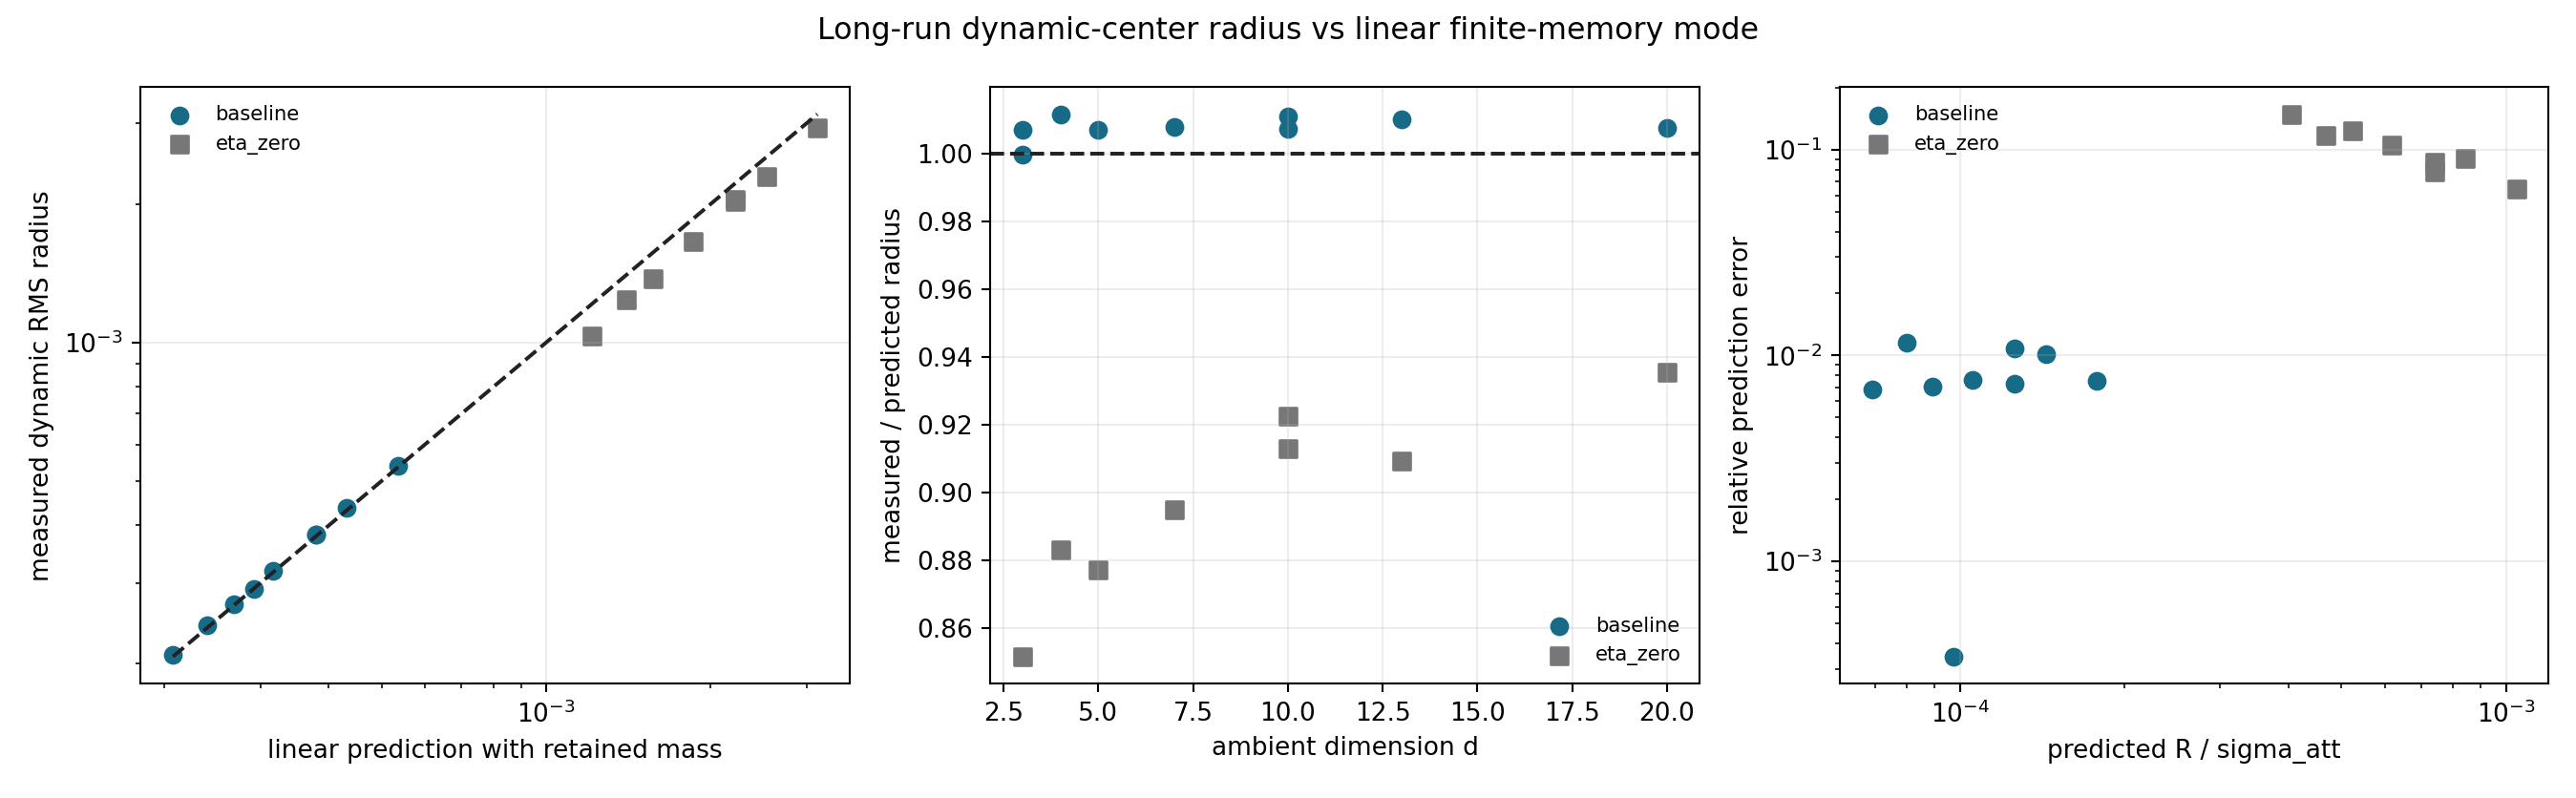
\includegraphics[width=\linewidth]{../../../figures/draft/scalar_hardening/linear_reconciliation_2026-07-19/linear_long_run_reconciliation.png}
    \caption{Measured co-moving root-mean-square radii compared with the
    finite-memory linear prediction. Active slices remain close to the
    diagonal across run length and ambient dimension. The $\eta=0$ controls
    are displayed separately because the active-force prediction is not an
    exact identity for their finite-window trace estimator.}
    \label{fig:linear_reconciliation_full}
\end{figure}

A matched kernel-family control sharpens this result.
For the earlier two-scale kernel, local curvature depends on the effective
amplitude $A_{\mathrm{eff}}=A_{\mathrm{att}}-9$ in the reference
normalization.
An attractive-only kernel at the same $A_{\mathrm{eff}}$ reproduces the
measured scalar radius, memory dimension, roundness, and center drift to
relative differences below $6.4\times10^{-6}$ over the matched support.
The compact branch therefore identifies local restoring curvature, not the
repulsive component of the two-scale kernel.

A preregistered fixed-$g$ test increased the predicted scale to
$R_{\mathrm{lin}}/L=0.3$.
Its endpoint radius is $6.2\%$ above the linear prediction, but the memory
shape changes only smoothly and no separate branch is resolved.
Fixed-voxel residence changes with the deliberately varied radius, while a
co-moving residence statistic is saturated for both active and $\eta=0$
paths.
The formal composite decision is therefore inconclusive and does not support a
metastable-transition claim.

The covariance participation dimension $D_{\mathrm{mem}}$ approaches the
supplied dimension for an isotropic cloud.
A value near three in a three-dimensional embedding is consequently an
expected shape check in this linear regime, not a dimension-selection result.
We do not use it as primary evidence.

\subsection{Terminology and discriminating tests}

We call the state established above a \emph{co-moving localized memory cloud}.
The project term \emph{dynamical knot} is reserved for a stronger result: a
nonlinear metastable regime that remains after comparison with
Eq.~(\ref{eq:relative_mode_full}), matched $\eta=0$ controls, and scale-aware
measurement choices.
The historical illustrative knot trajectory is therefore not used as evidence
in the revised paper.

For a region $\mathcal K\subset\Omega$, retained memory weight
\begin{equation}
M_n(\mathcal K)=\int_{\mathcal K}\rho_n(x)\,dx
\end{equation}
can contribute to such a test, but only if $\mathcal K$ is defined without a
fixed-bin scale bias and the same statistic does not saturate under the null.
Residence time, memory weight, and shape must be tested jointly across seeds
and controls.

A more direct metastability test estimates a lagged transfer operator on
features of the augmented state.
Almost-invariant sets or nontrivial slow modes should be stable under changes
of lag, basis or partition, terminal-row handling, and sample size
\cite{FroylandLloydSantitissadeekorn2010,NoeNuske2013,
NoeWuPrinzPlattner2013}.
For a non-unit eigenvalue $\mu_i(\tau)$, the implied rate is
\begin{equation}
\Gamma_i(\tau)=-\frac{1}{\tau}\log|\mu_i(\tau)|.
\label{eq:implied_rate_full}
\end{equation}
A slow eigenvalue is meaningful only if it is separated from finite-sample and
projection artifacts and from the corresponding control spectrum.

\subsection{Local relaxation diagnostics}

For a quasi-stationary memory field, let $x_\star$ satisfy
$\nabla\Phi[\rho](x_\star)=0$ and let $H$ be the Hessian of the memory
potential there.
The formal continuum approximation from Eq.~(\ref{eq:coarse_sde}) gives
\begin{equation}
dX_t=-\frac{\eta}{\alpha}H(X_t-x_\star)\,dt
     +\sqrt{2D}\,dW_t .
\label{eq:ou_full}
\end{equation}
Local restoring behavior requires the symmetric part of $H$ to be positive in
the directions considered.
If $\lambda_H$ is a characteristic eigenvalue, the frozen-memory rate scales
as
\begin{equation}
\Gamma_{\mathrm{rel}}\sim\frac{\eta}{\alpha}\lambda_H .
\end{equation}
This is a local approximation to the broader spectral diagnostic in
Eq.~(\ref{eq:implied_rate_full}), not an independent proof of a metastable
state.

A dimensionless comparison with diffusion on the deposition scale is
\begin{equation}
\widehat\Gamma=\frac{\sigma^2}{D}\Gamma_{\mathrm{rel}}.
\end{equation}
It is approximately invariant under uniform coordinate rescaling when
$\sigma$ and $D$ are transformed consistently.
Neither $\Gamma_{\mathrm{rel}}$ nor $\widehat\Gamma$ is a physical mass.
Such an interpretation would require a separate operational calibration that
is absent from this paper.
\section{Discussion and Outlook}
%-------------------------------------------------

We have specified a self-interacting stochastic process with an explicit
exponentially relaxing spatial memory field.
The visible coordinate is generally non-Markovian, while position plus the
full memory field form a Markov state.
The memory recursion supplies a finite persistence scale and a transparent
history compression; a continuum SDE is available only as a stated scaling
approximation.

The principal numerical conclusion is narrower and more informative than the
earlier knot interpretation.
The corrected scalar reference branch is a reproducible co-moving relaxation
cloud whose radius follows the exact linear center-relative prediction across
all nine tested long-run slices.
Kernel-family matching shows that the same branch identifies local restoring
curvature rather than a specifically two-scale mechanism.
The largest controlled departure found so far is a smooth $6.2\%$ radius
correction without a resolved shape or residence transition.
Accordingly, nonlinear metastability remains unestablished.

A separate finite-time stress test probes how far this conclusion transfers to
two previously admitted, prepared rotating waves in the deterministic
$d=2$ finite-memory branch.  Additive innovations were restored and compared
at fixed memory time through
\begin{equation}
\chi=\frac{\varepsilon}{R\sqrt{\alpha}},\qquad
\frac{D}{R^2}=\frac{\chi^2}{2}.
\label{eq:rotating_noise_coordinate_full}
\end{equation}
For both prepared cells and all three registered common-noise paths,
$10^{-15}\leq\chi\leq10^{-4}$ passed the finite-time orbital gates, whereas
$\chi=10^{-3}$ and $10^{-2}$ failed the preregistered local phase and
chirality gates.  The lower values $10^{-22}\leq\chi\leq10^{-16}$ were
numerically unresolved in the binary64 implementation.  Hence the result is
only the decade bracket
$10^{-4}\leq\chi_{\mathrm{stable}}<\chi_{\mathrm{fail}}=10^{-3}$; it is
neither an interpolated critical point nor evidence that the visible circles
disintegrate there.  Indeed, radius and transverse-deviation observables
remained well inside their gates at the first phase-coherence failure.  Raw
$\varepsilon$ is not transferable between cells or parameter conventions; in
these two cells its first failing values were $9.47\times10^{-5}$ and
$6.68\times10^{-5}$.  This prepared-orbit test does not establish noisy
formation, a stationary stochastic measure, or a physical noise calibration.

This result provides a baseline that future extensions must falsify rather
than merely fit.
A stronger claim requires a scale-aware almost-invariant set, a reproducible
nonlinear bifurcation, or a relational response absent from matched linear and
no-feedback controls.
The present model does not establish dimension selection, physical spacetime,
a hard signal speed, quantum dynamics, particle structure, or calibrated mass.
\bibliographystyle{apsrev4-2}
\bibliography{references}

\end{document}
